\section{【背景】X86的分页硬件支持}\label{ux80ccux666fx86ux7684ux5206ux9875ux786cux4ef6ux652fux6301}

X86
CPU对实际物理内存的访问是通过连接着CPU和北桥芯片的前端总线来完成的,在前端总线上传输的内存地址是物理内存地址。物理内存地址被北桥映射到实际的内存条中的内存单元相应位置上。然而,在CPU内执行带来软件所使用的是虚拟内存地址(也称逻辑内存地址),它必须被转换成物理地址后,才能用于实际内存访问。

前面已经讲过了80x86的分段机制,80x86的分页机制建立在其分段机制基础之上,提供了更加强大的内存管理支持。需要注意的是,在x86中,必须先有分段机制,才能有分页机制。在分段机制中,虚地址会转换为线性地址。如果不启动分页机制,那么线性地址就是最终在前端总线上的物理地址;如果启动了分页机制,则线性地址还会经过页映射被转换为物理地址。

那如果启动分页机制呢?在80x86中有一个CR0控制寄存器,它包含一个PG位,如果PG=1,启用分页机制;如果
PG=0,禁用分页机制。不像分段机制管理大小不固定的内存卡,分页机制以固定大小的存储块为最小管理单位,即把整个地址空间(包括线性地址和物理地址)都看成由固定大小的存储块组成。在80x86中,这个固定大小一般设定为4096字节。在线性地址空间中的最小管理单位(称为页(page)),可以映射到物理地址空间中的任何一个最小管理单位(称为页帧(page
frame))。页/页帧的32位地址由20位的页号/页帧号和12位的页/页帧内偏移组成。

80x86分页机制中的分页转换功能(即线性地址到物理地址的映射功能)需采用驻留在内存中的数组来描述,该数组称为页表(page
table)。每个数组项就是一个页表项。由于页/页帧基地址按4096字节对齐,因此页/页帧的基地址的低12位是0。页地址\textless{}-\textgreater{}页帧地址的转换过程以简单地看做80x86对页表的一个查找过程。页地址(线性地址)的高20位(即页号,or页的基地址)构成这个数组的索引值,用于选择对应页帧的页帧号(即页帧的基地址)。页地址的低12位给出了页内偏移量,加上对应的页帧基地址就最终形成对应的页帧地址(即物理地址)。

由于80x86的地址空间可达到4GB,按页大小(4KB)划分为1M个页。如果用一个页表来描述这种映射,那么该也表就要有1M个表项,若每个表项占用4个字节,那么该映射表就要占用4M字节。考虑到将来一个进程就需要一个地址映射表,若有多个进程,那地址映射表所占的总空间将非常巨大。为避免地址映射表占用过多的内存资源,80x86把地址映射表设定为两级。地址映射表的第一级称为页目录表,存储在一个4KB的物理页中,页目录表共有1K个表项,其中每个表项为4字节长,页表项中包含对应第二级表所在的基地址。地址映射表的第二级称为页表,每个页表也安排在一个4K字节的页中,每张页表中有1K个表项,每个表项为4字节长,包含对应页帧的基地址。由于页目录表和页表均由1K个表项组成,所以使用10位的索引就能指定表项,即用10位的索引值乘以4加基地址就得到了表项的物理地址。按上述的地址转换描述,一个页表项只需20位,但实际的页表项是32位,那其他的12位有何用途呢?

在80x86中的的页目录表项结构定义如下所示:

\begin{figure}[htbp]
\centering
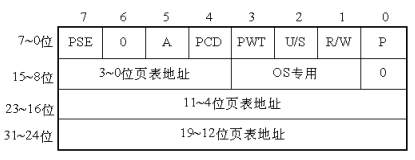
\includegraphics{figures/1.png}
\caption{1}
\end{figure}

在80x86中的的页表项结构定义如下所示:

\begin{figure}[htbp]
\centering
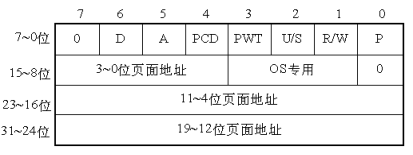
\includegraphics{figures/2.png}
\caption{2}
\end{figure}

其中低12位的相应属性位含义如下:

\begin{itemize}
\tightlist
\item
  P位:存在(Present)标志,用于指明此表项是否有效。P=1表示有效;P=0表示无效。如果80x86访问一个无效的表项,则会产生一个异常。如果P=0,那么除表示表项无效外,其余位用于其他用途(比如swap
  in/out中,用来保存已存储在磁盘上的页面的序号)。
\item
  R/W:读/写(Read/Write)标志,如果R/W=1,表示页的内容可以被读、写或执行。如果R/W=0,表示页的内容只读或可执行。当处理器运行在特权级(级别0、1或2)时,则R/W位不起作用。
\item
  U/S:是用户态/特权态(User/Supervisor)标志。如果U/S=1,那么在用户态和特权态都可以访问该页。如果U/S=0,那么只能在特权态(0、1或2)可访问该页。
\item
  A:是已访问(Accessed)标志。当CPU访问页表项映射的物理页时,页表项的这个标志就会被置为1。可通过软件把该标志位清零,并且操作系统可通过该标志来统计页的使用情况,用于页替换策略。
\item
  D:是页面已被修改(Dirty)标志。当CPU写页表项映射的物理页内容时,页表项的这个标志就会被置为1。可通过软件把该标志位清零,并且操作系统可通过该标志来统计页的修改情况,用于页替换策略。
\end{itemize}

下图显示了由页目录表和页表构成的二级页表映射架构。

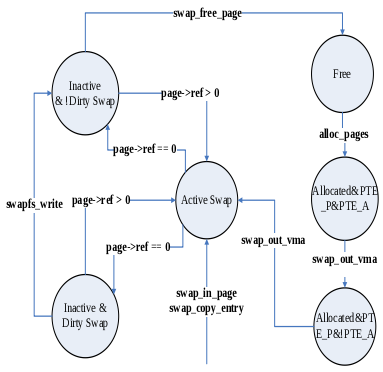
\includegraphics{figures/3.png} 图 页目录表和页表构成的二级页表映射架构

从图中可见,控制寄存器CR3的内容是对应页目录表的物理基地址;页目录表可以指定1K个页表,这些页表可以分散存放在任意的物理页中,而不需要连续存放;每张页表可以指定1K个任意物理地址空间的页。存储页目录表和页表的基地址是按4KB对齐。当采用上述页表结构后,基于分页的线性地址到物理地址的转换过程如下图所示:

首先,CPU把控制寄存器CR3的高20位作为页目录表所在物理页的物理基地址,再把需要进行地址转换的线性地址的最高10位(即22\textasciitilde{}
31位)作为页目录表的索引,查找到对应的页目录表项,这个表项中所包含的高20位是对应的页表所在物理页的物理基地址;然后,再把线性地址的中间10位(即12\textasciitilde{}21位)作为页表中的页表项索引,查找到对应的页表项,这个表项所包含的的高20位作为线性地址的基地址(即页号)对应的物理地址的基地址(即页帧号);最后,把页帧号作为32位物理地址的高20位,把线性地址的低12位不加改变地作为32位物理地址的低12位,形成最终的物理地址。

如果每次访问内存单元都要访问位于内存中的页表,则访存开销太大。为了避免这类开销,x86
CPU把最近使用的地址映射数据存储在其内部的页转换高速缓存(页转换查找缓存,简称TLB)中。这样在访问存储器页表之前总是先查阅高速缓存,仅当必须的转换不在高速缓存中时,才访问存储器中的两级页表。
